% !TEX root = ../master.tex
\chapter{Implementation}
\label{chap:impl}

The previous chapter yielded a general execution plan that shall implemented in the coming 
section while utilizing the cluster computer at the \ac{DHBW}. 
For each implementation detail the specifically chosen values are given during the process. Each of the steps holds 
the possibilities for errors which will also be evaluated.
The outcome of the taken steps is only a partially functional Hadoop cluster.
The reasons and implications for this restricted outcome are given.
Suggestions for future projects how better results might be achieved is given in the end.

\section{Infrastructure Set-Up in OpenStack}

\subsection{Preparation}

The foundation for the cluster architecture that has been illustrated in figure \vref{fig:architecture} are the host \acp{VM}, their storage and the network that connects them.
In the course of this process some minor adaptions are made to the proposed architecture.
Especially the \texttt{hadoop-master-0} node now also runs the \ac{HDFS} Datanode and YARN Nodemanager service and therefore has a storage volume attached to it.

To set up the cluster the web interface of OpenStack can be used, which is accessible at
\urlinline{https://controller.c4.dhbw-mannheim.de/} from within the \ac{DHBW} network.
Each operation on the infrastructure can be performed within this interface.

\subsection{Execution}

\subsubsection{Firewall Rules}

The firewall in OpenStack can be configured by creating \emph{security groups}.
These security groups describe rules for allowing and prohibit outgoing and incoming connections.
For this project two security groups are created and assigned to each of the \acp{VM}.
THe first group deals with \emph{default} settings. It allows all outgoing connections 
and allows incoming connections on port 22, which is the port used for \ac{SSH} access, 
as well as incoming ping packages in the Internet Control Message Protocol.
The second group deals with Hadoop specific ports.
A detailed over all necessary ports is given by \textcite{hortonworks2017reference} in their port reference.
However to make development and access more flexible, this group does temporarily 
allow all incoming requests.

\subsubsection{Network}

To enable an interconnection between the nodes in the cluster it is useful to create a private network between them.
The network uses the address space of 10.100.10.0/24 which is a subnet of the private address space defined in RFC~1918 by the the Internet Engineering Task Force \autocite[][]{ietf1996rfc1918}.
Figure \ref{fig:networks_subnets} lists all the networks that are available after the internal network is created. 
The network named \emph{int-net-10} is the internal network which all nodes connect to. Furthermore all nodes need to connect to the \emph{ext-net-201} network which allows them to connect to the Internet and makes them accessible from within the \ac{DHBW} network.

%\begin{table}[hbt]
%\resizebox{\textwidth}{!}{%
%	\begin{tabular}{lll}
%	  Network Name & Sub-networks & Description\\
%	  \hline
%	  ext-net-201 & 141.72.191.0/24 & Pre-configured connection to \ac{DHBW} internal network\\
%	  ext-net-112 & 192.168.112.0/20 & Pre-configured connection with unknown connectivity\\
%	  int-net-10 & 10.100.10.0/24 &  New internal network used by Hadoop\\
%	\end{tabular}%
%	}
%	\caption{Sub-networks within the project in OpenStack}
%	\label{fig:networks_subnets}
%\end{table}

\begin{figure}[hbt]
  {\centering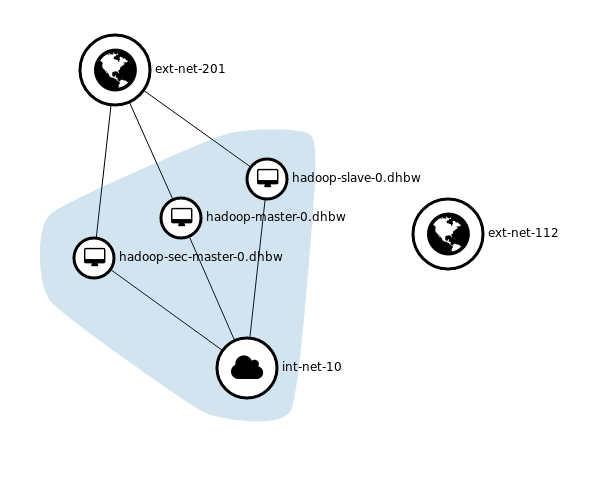
\includegraphics[width=0.8\textwidth]{{img/network_topology}.png}\par}
  \caption{Network topology created in OpenStack}
  \label{fig:network_topology}
\end{figure}

Once the nodes are created, the network topology looks like figure \ref{fig:network_topology}. The highlighted denotes the network connections that exists purely in OpenStack and have no physical connection to any outside network.
The figure also shows the names of the hosts and the network names.

\subsubsection{Virtual Machines}

In the next step the virtual machines are created.
The OpenStack environment offers different \emph{flavors} of instance sized for the \acp{VM} which is a pre-configured combination of resources associated to it.
To create a node the developer can chose from the presets listed in table \ref{fig:instance_sizes}. The flavors differ in amount of \acp{VCPU}, \ac{RAM} and root storage.
The set-up of the hosts is done for each node individually, 
since the names and flavor configurations differ between them.
The names are respective to proposed architecture but have a \emph{dhbw} domain ending 
added to them, which is not officially registered but is necessary for Ambari to identify the hosts correctly.


%\begin{table}[hbt]
%\centering
%\resizebox{0.8\textwidth}{!}{%
%	\begin{tabular}{lrrr}
%	  Instance Flavor Name & \acp{VCPU} & \acs{RAM} & Root Disk Size \\
%	  \hline
%	  m1.nano & 1 & 64~\acs{MB} & 1~\acs{GB} \\
%	  m1.tiny & 1 & 512~\acs{MB} & 5~\acs{GB} \\
%	  m1.small & 1 & 1~\acs{GB} & 10~\acs{GB} \\
%	  m1.medium & 2 & 2~\acs{GB} & 20~\acs{GB} \\
%	  m1.large & 4 & 4~\acs{GB} & 40~\acs{GB} \\
%	  m1.xlarge & 8 & 8~\acs{GB} & 80~\acs{GB} \\
%	\end{tabular}%
%	}
%	\caption{Available instance sizes in the \ac{DHBW} OpenStack environment}
%	\label{fig:instance_sizes}
%\end{table}


%\begin{table}[hbt]
%\centering
%	\begin{tabular}{lrl}
%	  Resource Type & Amount & Unit\\
%	  \hline
%	  Instances & 10 & \\
%	  \acp{VCPU} & 20 & \\
%	  \acs{RAM} & 51200 & \acs{MB} \\
%	  Floating \acs{IP} Addresses & 10 & \\
%	  Security Groups & 10 & \\
%	  Volumes & 10 & \\
%	  Volume Storage & 1000 & \acs{GB}
%	\end{tabular}
%	\caption{Available resources for the project in the \ac{DHBW} OpenStack environment}
%	\label{fig:resources_openstack}
%\end{table}

Table \ref{fig:resources_openstack} describes how many resources are available at maximum for the project in the \ac{DHBW} OpenStack environment. The chosen configurations may in sum not exceed this limit.
As visible in table \ref{fig:instance_sizes} all instance of m1.small and larger have a core to memory ration of \emph{1~core~:~1~GB~RAM}, which means that, if all 20 available cores are used, only 20 out of 51.2 GB RAM  can be used. It is favourable to have maximum sized \acp{VM} with respect to memory to give Hadoop the possibility make better use of it.
Therefore the best allocation for the nodes is to use a m1.xlarge instance for the master node, a m1.xlarge for the secondary and a large instance for the slave node.
This in sum gives 20 \acp{VCPU} and 20~\ac{GB} \ac{RAM} and no further cores are available to allocate more nodes.


Each instance is using the Ubuntu 16.04 operating system which is compatible with \ac{HDP}, Ambari and Hadoop. As discussed before the security groups for default access and hadoop specific access are assigned to the hosts, and they are connected to the internal and external network. An \ac{SSH} key is used for authentication.
The successful creation of each host is tested by accessing it via \ac{SSH} using the specified key and the user \emph{ubuntu}.


\subsubsection{Storage}

In order for the Hadoop cluster to store \ac{HDFS} data it is necessary to split up the available 1000~\ac{GB} for storage into three volumes, one for each host.
The disks are attached to the hosts and OpenStack reports the device handle that can be 
used within the hosts to access the volume.
Before data can be stored on the volumes they each need to be partitioned into one partition using the program \texttt{fdisk}. The partitions are then formatted into ext4 file system format using the \texttt{mkfs.ext4} command.

\subsection{Encountered Issues and Lessons Learned}

Access to the OpenStack environment and the cluster nodes is only possible from within the \ac{DHBW} network that connects the \ac{DHBW} Mannheim and Stuttgart.
This network is not accessible via an virtual private network and the developer needs to be on premise of the \ac{DHBW}. This restriction in locality makes the development process harder.

During the implementation, the OpenStack environment showed significant instabilities.
\emph{Internal errors} lead in some cases to the failure of allocation of resources for the requested \acp{VM}.
This might indicate an general shortage of resources in the \ac{DHBW} OpenStack environment. Later in the project these internal errors have been resolved.

\section{System Set-Up with Ansible}

TODO ansible script already used in chapter 3 so now it is adapted to the new needs

\subsection{Preparation}

TODO
TODO explain and maybe print this particular playbook yes yes print it with explainations
TODO maybe appendix
TODO Ansible
also install ansible localy


The full Ansible playbook including all roles and templates is stored on the authors \emph{GitHub repository} and can be accessed at 
\urlinline{https://github.com/XOSplicer/studienarbeit-hadoop-cluster-ansible}.

TODO describe all roles and task within those roles

\subsubsection{Common Set-Up Tasks}

\subsubsection{Specific Tasks for Ambari Server}

\subsubsection{Specific Tasks for Ambari Client}
     


\subsection{Execution}

TODO enter ssh config

Before a host can be used with Ansible, it needs to have \emph{Python 2} installed.
Therefore a short script cat be run on each host, which updates the system, installs Python and reboots the system. This ensures all packages are up to date. The following bash script performs these tasks and also installs the \emph{python-apt} library which is necessary for Ansible to install more packages.

\lstset{language=sh}
\begin{lstlisting}[caption={Bash script for initial host preparation}, label={lst:hostsetup}]
sudo apt-get update \&\& sudo apt-get -y upgrade
sudo apt-get -y install python2.7 python-apt
sudo reboot now
\end{lstlisting}

After this initial preparation of the hosts is done, 
the Ansible inventory can is configured, 
so that all the specific variables of the host are set. 
These variables are the \ac{FQDN}, the internal \ac{IP} address, 
the network interface that is connected to the internal network 
and finally the \ac{UUID} of the partition that is used to store the \ac{HDFS} data.

The \ac{FQDN} is again taken from the \texttt{ssh\_config} file. 
The internal \ac{IP} address is taken from the OpenStack web interface.
To find the values for the other variables each host is accessed.
The internal network interface is the second Ethernet interface listed with the command \texttt{\$ ifconfig -a}. Typically it is called \texttt{ens4}, \texttt{ens6} or \texttt{ens7}.
The \ac{UUID} of the storage volume is found by running \texttt{\$ sudo blkid}. 
It reports the \ac{UUID} of all volumes. The one corresponding to the device that has been created in OpenStack can be found in the output. These variables are then entered into the \texttt{inventory.ini} file for Ansible. The master node is entered in the \texttt{master} section, the slave nodes in the \texttt{slave section respectively}.

\lstset{language=sh}
\begin{lstlisting}[caption={Inventory description in Ansible}, label={lst:inventory}]
[master]
hadoop-master-0.dhbw internal_ip=10.100.10.24 iface_internal=ens4 hadoop_vol_uuid=47103a5e-5c3f-40f3-a710-fcd86e23fc61

[slave]
hadoop-sec-master-0.dhbw internal_ip=10.100.10.25 iface_internal=ens4 hadoop_vol_uuid=54b1d167-9b88-45c1-b27f-6e441b765c66
hadoop-slave-0.dhbw internal_ip=10.100.10.26 iface_internal=ens4 hadoop_vol_uuid=046a2bc2-df33-4640-becd-2c401076285f
\end{lstlisting}


Now all necessary variables are set and the Ansible playbook is be applied to the hosts.
This is done using the command \texttt{\$ ansible-playbook all}.
Ansible connects to each of the hosts and performs the neccessary stept to get the 


TODO apply ansible playbook
reboot for safty

\subsection{Encountered Issues and Lessons Learned}

TODO
literary none?
Ansible is very capable to perform system administration tasks in a reproducable fashion

\section{Hadoop Set-Up with Ambari}

\subsection{Preparation}

After the Ambari software is installed on each host by Ansible, it can be utilized to set-up the Hadoop cluster and install additional tools as well.
To do so the Ambari web interface is used that can be accessed on the master node on port 8080. The complete Hadoop setup is performed using the cluster deployment dialogue that Ambari offers. This process follows the execution plan closely.

\emph{Jonas Balsfulland} proposes in his paper which additional tools should be running on the cluster. Especially \emph{Spark 2, Storm, Hive and Pig} should be deployed.
Ambari offers the possibility to set up all of these services automatically if they are selected during the cluster setup.

\subsection{Execution}

The deployment dialogue in Ambari guides the user through the cluster installation.
For this project a cluster named \emph{hadoopdhbw0} is created which installs \ac{HDP} Version 2.6.3.0. All binary packages are downloaded from Hortonworks repositories.
The list of the \acp{FQDN} including the \emph{dhbw} domain of the three \acp{VM} are entered as cluster nodes. They are registered using \emph{manual registration} since the Ambari agent installed on all nodes is configured to contact the master node as the Ambari server. Furthermore this elides the necessity to upload an unencrypted \ac{SSH} key with root access to the servers.
Ambari then checks the connectivity to each host and performs preliminary checks about the host that ensure the cluster can be deployed successfully.

Next the services and additional tools are chosen which are installed on the cluster.
For this setup \ac{HDFS}, \ac{YARN}, MapReduce2, Tez, Hive, Pig, ZooKeeper, Storm, SmartSense, Spark2, Slider and Ambari Metrics are selected. SmartSense, Slider, ZooKeeper and Ambari Metrics are enforced to be installed by Ambari.


TODO firther installation


TODO In the end Ambari monitoring web interface used to inspect the cluster and the services

TODO some are failing, needs often restart etc

\subsection{Encountered Issues and Lessons Learned}

During the initial evaluation of Ambari in section \vref{sec:design:hdp_ambari_ansible} it was figured that 20~\ac{GB} of root storage for the installation of the cluster is not enough. This approach uses a reduced set of services that are installed which leads to less disk space needed. Therefore the 80~\ac{GB} root volume is sufficient on all nodes as expected previously.

During the installation process several issues regarding domain name resolution appeared.
This is caused by the fact that no proper \ac{DNS} server is used to distribute the \acp{FQDN} 
but rather the \texttt{hosts} file is altered in a way that the resolution works locally between all nodes. 
This holds the possibility for configuration errors which lead which lead to the failure of the installation at first.
The issues are fixed by adapting the \texttt{hosts} file to only perform name resolution for the selected \acp{FQDN} for the local, internal network. 

One major issue is encountered when Ambari tries to start all services: The main memory on the master node, which is limited to 8~\ac{GB} is not sufficient and the system is instable.
When the master node runs out of memory the operating system can kill arbitrary services that are running
Since this is happening on the master node, this leads to the service not being available at all.
Therefore some services are turned of explicitly. In particular Hive, SmartSense and Spark2 are deactivated for the entire cluster. 
This way the master node has enough memory to run the other services.

\section{System Tests}

Before the processing system can be tested a new directory to store the test data in \ac{HDFS}
is created. 
This folder is \texttt{/user/ubuntu} and is accessible by the user \texttt{ubuntu}.
To test this step a new file is uploaded to the directory and its content is then downloaded again which tests successful. The directory is used in the next step.

\subsubsection{Terasort}

As suggested in the execution plan the \emph{terasort} program implemented by \textcite{omally2008terasort}, which is included in the Hadoop installtion on each cluster node, is used to check the sanity of the \ac{YARN}, \ac{HDFS} and MapReduce2 Services.
First \emph{teragen} generates a variable amount of random numbers and stores them on \ac{HDFS}. Then \emph{terasort} sorts the numbers using MapReduce and stores the result.
Finally \emph{teravalidate} checks that the numbers are indeed sorted correctly.
To run the test the follig commands are used to create 5~\ac{GB} fo data:\\

\lstset{language=sh}
\begin{lstlisting}[caption={Running Terasort as a test for YARN and HDFS}, label={lst:terasort}]
hadoop jar hadoop-mapreduce-examples.jar teragen 5000000 /user/ubuntu/test/5gsort/input
hadoop jar hadoop-mapreduce-examples.jar terasort /user/ubuntu/test/5gsort/input /user/ubuntu/test/5gsort/output
hadoop jar hadoop-mapreduce-examples.jar teravalidate /user/ubuntu/test/5gsort/output
\end{lstlisting}

The test are done for 1~\ac{MB}, 1~\ac{GB} and 5~\ac{GB}.
All test finish successfully, which means that MapReduce jobs can be successfully scheduled on the cluster and can interact with \ac{HDFS}.

\subsubsection{Ambari Service Checks}

Ambari offers the possibility to run \emph{service checks}, which run a small workload on one service and makes sure the cluster behaves correctly.
These checks are run in this project for all services that are active.
The services that are inactive due to memory shortage can not be tested.
The checks are therefore performed  only for \ac{HDFS}, \ac{YARN}, MapReduce2, ZooKeeper, Storm, and Ambari Metrics. All of the checks are giving successful results, which only means the service works as expected. It does not show that all nodes are participating in the cluster for this service. 

\section{Conclusion}

In general the cluster installation is only partially successful since the services are not running reliably and some even are not active at all due to memory limitations.
The produced cluster is therefore not ready for \emph{production use}.
However the general concept of using OpenStack to host the cluster and Ansible and Ambari to deploy the cluster software and manage Hadoop is possible and has clearly advantages above a manual cluster management.

During the project the \ac{DHBW} Cloud environment showed unreliabilities that influenced the progress of the implementation phase.
The general process was errorsome and would be hard to reproduce for students or lecturers with little knowledge about system administration. It is therefore not recommended to pursue a installation of Hadoop within the context of a lecture. 


















